\documentclass[11pt,a4paper]{article}
\usepackage[margin=22mm]{geometry}
\usepackage{amsmath,booktabs,graphicx,hyperref}
\title{CSA performance with direct carrier collection}
\date{\today}
\begin{document}\maketitle
\section{Inputs and unchanged circuit}
The corrected ion histories assign sampled Gaussian carrier positions directly
to physical pixels and time buckets. The historical histories assigned occupied
diffusion-cell centres to those grids. Both versions use 8000 events per sample.
Checks confirm identical source event IDs, event seeds, sampled drift distances,
diffusion widths and produced carrier counts. Each file passes its independent
collected/retained/outside ledger checks. The configurations are 2 mm pitch with
20 ms frames and 4 mm pitch with 40 ms frames.

The electronics are unchanged: 180 nm optimized CSA, external capacitance
1.25 pF, $C_f=3$ fF, grounded feedback gate with $M_f$ width 0.36 $\mu$m and
length 400 $\mu$m, and $M_4$ gate at 0.6164 V. Five-ms centred averages are
compared using the same fixed low-charge gain and fitted discharge correction.
Nominal quiescent ENC remains 61.3 electrons at 20 ms and 75.8 at 40 ms.

Input currents use uniform collection times within each saved bucket. The
single-ion current remains the constant-speed final approach at 3 m/s over a
5 mm gap to a 0.5 mm square pad in a grounded plane. Its integral is
$e[1-\phi_w(g)]$ per ion. Event simulations start at the quiescent operating
point. No random noise is added to the mean transient responses.

\section{Coverage}
\begin{center}\scriptsize\begin{tabular}{llrrrr}\toprule
Sample & Input & Events & Occupied cells & Simulated pads & Controls\\\midrule
2 mm / 20 ms, $0\nu\beta\beta$ & historical & 8,000 & 12,316,142 & 386 & 48 \\
2 mm / 20 ms, $0\nu\beta\beta$ & direct & 8,000 & 13,334,119 & 55 & 48 \\
2 mm / 20 ms, electrons & historical & 8,000 & 14,209,869 & 489 & 48 \\
2 mm / 20 ms, electrons & direct & 8,000 & 15,841,990 & 50 & 48 \\
4 mm / 40 ms, $0\nu\beta\beta$ & historical & 8,000 & 2,676,238 & 2,193 & 48 \\
4 mm / 40 ms, $0\nu\beta\beta$ & direct & 8,000 & 2,776,437 & 1,770 & 48 \\
4 mm / 40 ms, electrons & historical & 8,000 & 3,182,867 & 1,713 & 48 \\
4 mm / 40 ms, electrons & direct & 8,000 & 3,354,240 & 1,186 & 48 \\
\bottomrule\end{tabular}\end{center}
The complete linear screen retains every pad and empty frame. The nonlinear
batch simulates every history with a predicted minimum below 0.35 V, together
with twelve fixed-seed controls in each higher-voltage stratum per sample.
The separate twelve-case study retains matched baselines and two resolutions.

\section{Input pulses}
\begin{center}\small\begin{tabular}{llrrrr}\toprule
Sample & Input & Mean ions/cell & Median & Mean event mean & Maximum\\\midrule
2 mm / 20 ms, $0\nu\beta\beta$ & historical & 72.8 & 14 & 122.9 & 30,633 \\
2 mm / 20 ms, $0\nu\beta\beta$ & direct & 67.3 & 14 & 82.9 & 11,828 \\
2 mm / 20 ms, electrons & historical & 63.1 & 13 & 135.7 & 32,492 \\
2 mm / 20 ms, electrons & direct & 56.6 & 12 & 70.5 & 9,531 \\
4 mm / 40 ms, $0\nu\beta\beta$ & historical & 335.2 & 45 & 408.5 & 30,633 \\
4 mm / 40 ms, $0\nu\beta\beta$ & direct & 323.1 & 43 & 375.0 & 21,401 \\
4 mm / 40 ms, electrons & historical & 281.9 & 40 & 366.7 & 32,492 \\
4 mm / 40 ms, electrons & direct & 267.5 & 38 & 311.6 & 22,207 \\
\bottomrule\end{tabular}\end{center}
These means and medians refer to positive pad/frame cells across the sample.
They differ from an average of per-event means, which is also saved in the
comparison HDF5. No charge threshold is applied.

\section{Confirmed event compression}
Relative response loss compares the nonlinear and linear frame signals for the
same pad history. A bucket is flagged when it contains collected ions and
exceeds both the selected fractional loss and one nominal ENC of missing
signal. An event is counted once if any tested pad contains a flagged bucket.

\begin{center}\scriptsize\begin{tabular}{llrrrr}\toprule
Sample & Input & $\geq10\%$ & $\geq25\%$ & $\geq50\%$ & $\geq75\%$\\\midrule
2 mm / 20 ms, $0\nu\beta\beta$ & historical & 2.013 & 1.337 & 0.900 & 0.625 \\
2 mm / 20 ms, $0\nu\beta\beta$ & direct & 0.088 & 0.025 & 0.000 & 0.000 \\
2 mm / 20 ms, electrons & historical & 2.900 & 2.250 & 1.512 & 0.838 \\
2 mm / 20 ms, electrons & direct & 0.025 & 0.013 & 0.000 & 0.000 \\
4 mm / 40 ms, $0\nu\beta\beta$ & historical & 15.937 & 8.287 & 4.050 & 1.487 \\
4 mm / 40 ms, $0\nu\beta\beta$ & direct & 13.025 & 6.588 & 2.763 & 0.675 \\
4 mm / 40 ms, electrons & historical & 13.000 & 7.300 & 3.962 & 1.300 \\
4 mm / 40 ms, electrons & direct & 9.287 & 4.638 & 2.087 & 0.413 \\
\bottomrule\end{tabular}\end{center}
Entries are percentages of each full 8000-event sample. They count confirmed
cases in the conservative screened study and its controls. A flag identifies
local distortion; event usefulness will be evaluated with reconstructed tracks.
Zero observed flags in the tested 2 mm cases is an empirical result for this
sample and screening coverage.

\begin{figure}[ht]\centering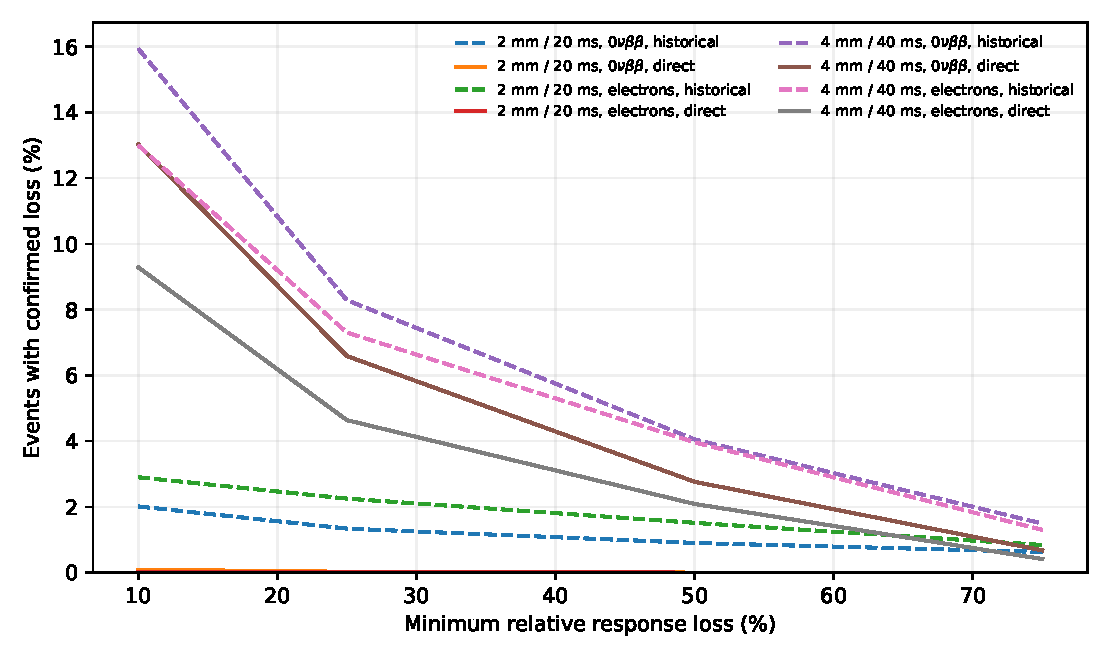
\includegraphics[width=\linewidth]{compression_comparison.pdf}
\caption{Historical and direct-collected inputs, evaluated with the same circuit
and one-ENC missing-signal criterion.}
\end{figure}

\section{Event 3790}
\begin{center}\begin{tabular}{lrr}\toprule
Electron input & Event buckets & Occupied buckets across all pads\\\midrule
historical & 502 & 15 \\
direct & 507 & 65 \\
\bottomrule\end{tabular}\end{center}
The extended arrival interval follows the source event geometry. Direct
collection fills the numerical gaps introduced by coarsening the diffusion
cloud before readout. Each plotted axis begins at that dataset's first retained
slice; the reference shifts slightly when the binned approximation is removed.
\begin{figure}[ht]\centering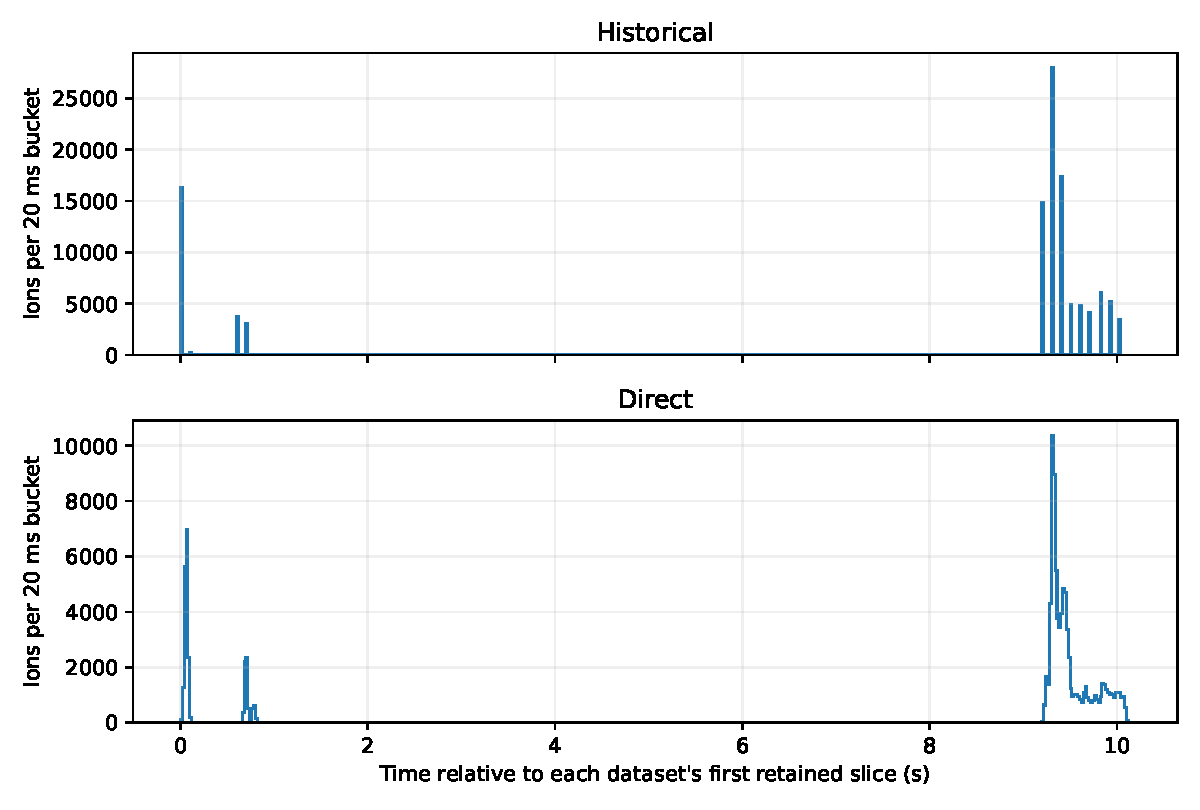
\includegraphics[width=\linewidth]{event_3790.pdf}
\caption{Full-event collected counts before and after the numerical correction.}
\end{figure}

\section{Reproduction}
From the repository root:
\begin{verbatim}
python scripts/run_pad_history_pipeline.py \
  --config config/pad_history_readout_direct.toml \
  --simulator /path/to/LTspice
python scripts/run_pad_compression.py \
  --config config/pad_history_viewer_direct.toml --workers 4
julia --project=. scripts/electronics/histories/compare_inputs.jl
python scripts/electronics/histories/present_input_comparison.py
python scripts/view_pad_histories.py
\end{verbatim}
Julia writes \texttt{results/ltspice/pad\_history\_direct\_comparison/comparison.h5};
Python presents its saved values. The source files, configurations, screen
outputs and nonlinear statistics have recorded hashes. Historical results are
preserved, and the corrected viewer uses the direct-input configuration by
default. The report source is generated without compiling a PDF.
\end{document}
